 \documentclass[xcolor=dvipsnames,table]{beamer}

\usepackage{latexsym}
\usepackage[utf8]{inputenc}
\usepackage[brazil]{babel}
\usepackage{amssymb}
\usepackage{amsmath}
\usepackage{stmaryrd}
\usepackage{fancybox}
\usepackage{datetime}
\usepackage[T1]{fontenc}
\usepackage{graphicx}
\usepackage{graphics}
\usepackage{url}
\usepackage{algorithmic}
\usepackage{algorithm}
\usepackage{acronym}
\usepackage{array}

\newtheorem{definicao}{Definio}
\newcommand{\tab}{\hspace*{2em}}

\mode<presentation>
{
  \definecolor{colortexto}{RGB}{0,0,0}
 
  \setbeamertemplate{background canvas}[vertical shading][ bottom=white!10,top=white!10]
  \setbeamercolor{normal text}{fg=colortexto} 

  \usetheme{Warsaw}
}

\title{Apresentação da Disciplina}  

\author{
  Esdras Lins Bispo Jr. \\ \url{bispojr@ufj.edu.br}
  } 
 \institute{
  Tópicos em Informática e Educação \\Bacharelado em Ciência da Computação}
\date{\textbf{18 de março de 2026} }

\logo{
\includegraphics[width=1.5cm]{images/ufjJataiLogo.png}}

\begin{document}

	\begin{frame}
		\titlepage
	\end{frame}

	\AtBeginSection{
		\begin{frame}{Sumário}%[allowframebreaks]{Sumário}
    		\tableofcontents[currentsection]
    		%\tableofcontents[currentsection, hideothersubsections]
		\end{frame}
	}

	\begin{frame}{Plano de Aula}
		\tableofcontents
		%\tableofcontents[hideallsubsections]
	\end{frame}
	
	\section{Sobre a Disciplina}
	\subsection{Professor}
	\begin{frame}{Professor}
		\begin{columns}
			\column{.4\textwidth}  		
			\begin{center}
				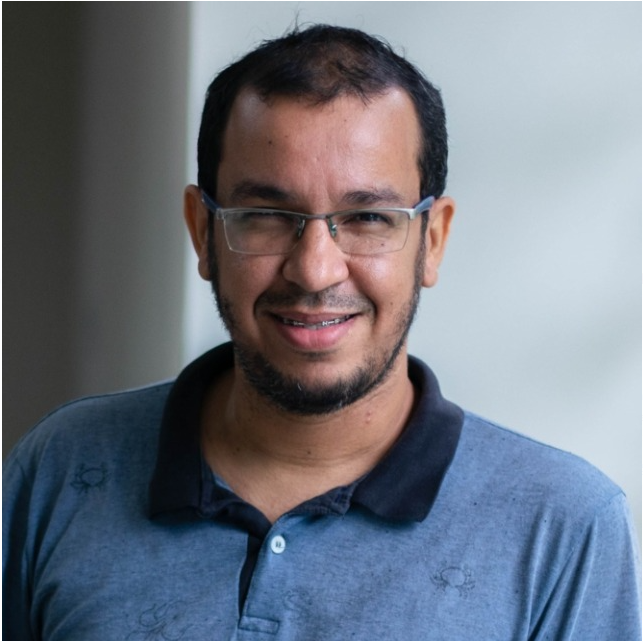
\includegraphics[height=.5\textheight]{images/eu-quadrado.png}
			\end{center}
			\column{.6 \textwidth}  		
			\begin{block}{Quem?}
				\begin{center}
					{\bf Esdras Lins Bispo Junior} \\ Recife, Pernambuco.
				\end{center}
			\end{block}
			\begin{block}{Formação}
				\begin{center}
					{\normalsize Sistemas de Informação (Grad.)\\
                    Inteligência Artificial (Mest.)\\
                    Educação em Computação (Dout.)}
				\end{center}
			\end{block}	
			\begin{block}{Linha de Pesquisa}
				Equidade na Educação em Computação
			\end{block}
		\end{columns}
	\end{frame}
	
	\subsection{Informações Importantes}
	\begin{frame}{Informações Importantes}
		\begin{block}{Professor}
			\begin{itemize}
				\item Esdras Lins Bispo Jr.
				\item \url{bispojr@ufj.edu.br}
				\item Sala 18, 1º Andar (Bloco dos Professores, próx. CA2)
			\end{itemize}
		\end{block}
	\end{frame}	
	
	\begin{frame}{Informações Importantes}
		\begin{block}{Disciplina}
			\begin{itemize}
				\item Tópicos em Informática e Educação (ICE 0648)
				\item 13h30-15h10 (Segunda, [CA1, Sala 5])\\
				 13h30-15h10 (Quarta, [CA1, Anfiteatro Superior])
				\item Dúvidas: 15h10 (Quarta)\\
				{\color{red}[é necessário confirmação comigo]}
				%\item Google Clasroom: Código - {\color{blue} \bf sufpjv5}
				\item Repositório: {\bf \color{red} ???}
			\end{itemize}
		\end{block}
	\end{frame}	
	
\begin{frame}{Informações Importantes}
    \begin{block}{Metodologia}
        \begin{itemize}
            \item Instrução pelos Colegas (IpC);
            \item Exercícios em Sala;
            \item Orientações individuais;
            \item Atividades em grupo (Projeto);
            \item Avaliação predominantemente formativa.
        \end{itemize}
    \end{block}
\end{frame}

	\begin{frame}{Plickers}
	\begin{center}
		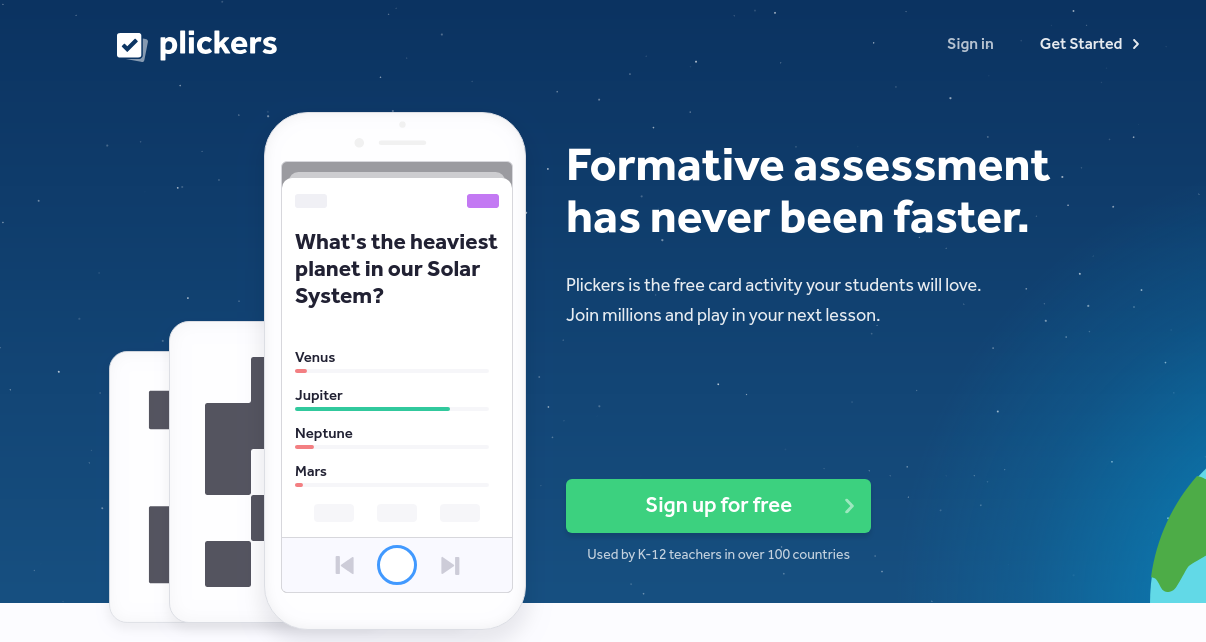
\includegraphics[width=\textwidth]{images/plickers}
	\end{center}
\end{frame}
	
	\begin{frame}{Metodologia IpC}
		\begin{center}
			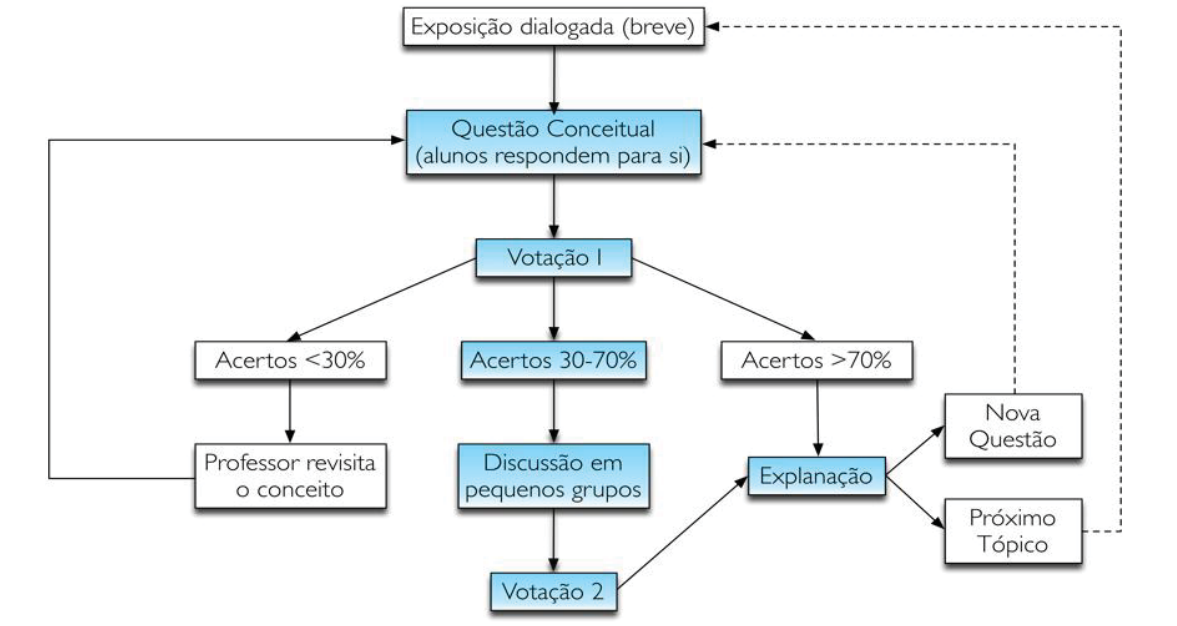
\includegraphics[height=.7\textheight]{images/fluxo-ipc}
		\end{center}
	\end{frame}

		\begin{frame}{Rotina Acadêmica}
			\begin{block}{Estudo Prévio}
				Antes de cada aula, haverá um material disponível para estudo prévio.
			\end{block}	\pause		
			% \begin{block}{{\it Quiz} (QZ)}
			% 	Antes de cada aula, será necessário responder a um {\it quiz} sobre o conteúdo a ser trabalhado.
			% \end{block} \pause
			\begin{block}{Questões Conceituais IpC (QC)}
				Toda aula haverá questões conceituais abordadas em sala.
			\end{block}
		\end{frame}

\section{Avaliação}
\subsection{Perspectivas}
\begin{frame}{Perspectivas sobre Avaliação}
    \begin{block}{Gestor x Formador}
        \begin{itemize}
            \item Gestor $\Rightarrow$ Excelência;
            \item Formador $\Rightarrow$ Aprendizagem.
        \end{itemize}
    \end{block} \pause
    \begin{exampleblock}{Qual é a principal função do professor?}
        \begin{itemize}
            \item Promover a excelência ou a aprendizagem?
            \item Parceiro ou Juiz?
        \end{itemize}
    \end{exampleblock}
\end{frame}

\begin{frame}{Avaliação Formativa}
    \begin{block}{Foco da Avaliação (PPC)}
        ``A avaliação deverá enfatizar o {\bf processo formativo} em detrimento da modalidade classificatória, desvinculando-se do âmbito da promoção/retenção para o âmbito da observação, do diagnóstico, acompanhados de registros sistemáticos de situações formais e informais'' (BCC, 2022, p. 67).
    \end{block} 
    \begin{exampleblock}{Projeto Pedagógico do Curso (PPC)}
        PPC | Bacharelado em Ciência da Computação (BCC):
        \url{https://computacao.jatai.ufg.br/p/3492-documentos}
    \end{exampleblock}
\end{frame}

\begin{frame}{Avaliação Formativa}
	\begin{center}
		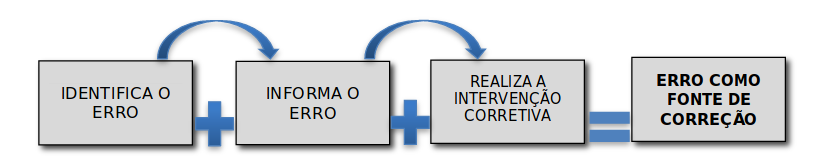
\includegraphics[width=\textwidth]{images/fluxo-correcao} \pause
		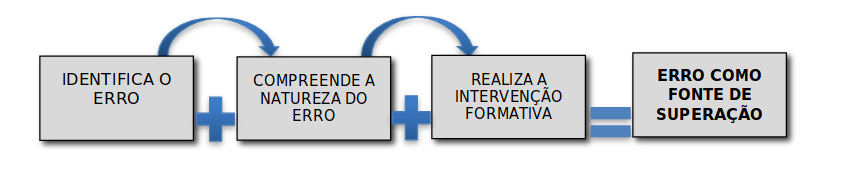
\includegraphics[width=\textwidth]{images/fluxo-superacao}
	\end{center}
\end{frame}

\begin{frame}{Avaliação Formativa}
    \begin{block}{Foco da Avaliação (PPC)}
        ``A avaliação deve servir, em primeiro lugar, para {\bf reorientar o aprendiz} no desenvolvimento das aprendizagens e o professor, no replanejamento das atividades. Não pode ser, pois, meramente classificatória, mas uma ferramenta construtiva, que promove melhorias e inovações, com vistas ao {\bf aperfeiçoamento da aprendizagem}. Aos alunos, após discussão sobre o processo, os instrumentos e os resultados da avaliação, devem ser propiciados meios que lhes permitam sanar dificuldades evidenciadas e realizar as aprendizagens em níveis crescentes de desenvolvimento.'' (BCC, 2022, p. 67).
    \end{block}
\end{frame}

\subsection{Instrumentos}

\begin{frame}{Instrumentos de Avaliação}
    \begin{block}{Critérios de Aprovação}
    	\begin{itemize}
    		\item Estar presente em 75\% dos nossos encontros;
    		\item Compromisso com a própria aprendizagem ($\cong$ 2h);
    		\item Engajamento na condução do projeto.
    	\end{itemize}
    \end{block} \pause
    \begin{exampleblock}{Nota Final}
    	Média Final = 6,0 + Autoavaliação Dialogada [0,0 a 4,0]
    \end{exampleblock}
\end{frame}

\begin{frame}{Instrumentos de Avaliação}
    \begin{block}{Motivos para Sinalizar o Descomprometimento}
        \begin{itemize}
            \item Por você (potencial humano)
            \item Pela turma (garantia do direito)
            \item Pela sociedade (prestação do uso do recurso)
        \end{itemize}
    \end{block}
\end{frame}

\begin{frame}{Instrumentos de Avaliação}
    \begin{alertblock}{Critérios de Reprovação}
        \begin{itemize}
            \item Ausência em 25\% dos nossos encontros ou mais;
            \item Descomprometimento com a própria aprendizagem durante à condução do projeto.
        \end{itemize}
    \end{alertblock} \pause
    \begin{block}{Nota Final}
        \begin{itemize}
            \item Média Final = 4,0.
        \end{itemize}
        
    \end{block}
\end{frame}

% 	\begin{frame}{Instrumentos de Avaliação}
	
% 	\begin{block}{Prova Final (PF) - 20\% da pontuação total}
% 		A PF é composta por duas etapas: a PF$_1$ e a PF$_2$. 
% 		A PF$_1$ é composta por dois mini-testes de caráter substitutivo: \pause 
% 		\begin{itemize}
% 			\item o SMT$_1$ (referente ao MT$_1$), e 
% 			\item o SMT$_2$ (referente ao MT$_2$).
% 		\end{itemize} \pause
% 		Por sua vez, a PF$_2$ é composta pelos outros dois mini-testes também de caráter substitutivo:  \pause
% 		\begin{itemize}
% 			\item o SMT$_3$ (referente ao MT$_3$), e 
% 			\item o SMT$_4$ (referente ao MT$_4$).
% 		\end{itemize}
% 	\end{block}
% \end{frame}

% \begin{frame}{Avaliação}
% 	\begin{block}{Média Final}
% 		O cálculo da média final será dada da seguinte forma:
% 		\begin{itemize}
% 			\item MF = MIN(10, PONT)
% 		\end{itemize}
% 		em que MIN representa o mínimo entre dois valores e PONT representa a pontuação total obtida em toda a disciplina, dada da seguinte forma:
% 		\begin{center}
% 			PONT = $\left[ \sum\limits_{i=1}^{4} \mbox{max}(MT_i, SMT_i) + PF \right] \times 0,2 + QC + QZ$
% 		\end{center}
% 	\end{block} \pause
% 	\begin{exampleblock}{Previsão de Término das Atividades}
% 		10 de julho de 2025
% 	\end{exampleblock}
% \end{frame}

\section{Conteúdo da Disciplina}
\begin{frame}{Conteúdo da Disciplina}
    \begin{block}{1. Introdução}
        \begin{enumerate}
            \item[a)] Por que esse encontro entre a Informática e Educação (I\&E)?
            \item[b)] Informática na Educação (IE)
            \item[c)] Educação em Computação (EC)
            \item[d)] Tecnologias na Educação em Computação: IE + EC
        \end{enumerate}
        
    \end{block}  \pause


    \begin{block}{2. Teorias Educacionais em I\&E}
        \begin{enumerate}
            \item[a)] Grandes Perspectivas: Pedagogia Liberal e Progressista
            \item[b)] Neutralidade e I\&E
            \item[c)] Pedagogia Tradicional e Tecnicista
            \item[d)] Pedagogia Libertadora e Crítico-Social dos Conteúdos
        \end{enumerate}
        
    \end{block}
\end{frame}

\begin{frame}[shrink]{Conteúdo da Disciplina}

        \begin{block}{3. Projetos em I\&E}
            \begin{enumerate}
                \item[a)] Tipos de Projetos em I\&E
                \item[b)] Projetos de Ensino em I\&E
                \item[c)] Projetos de Pesquisa em I\&E
                \item[d)] Projetos de Extensão em I\&E
                \item[e)] Projetos de Inovação em I\&E
            \end{enumerate}
            
        \end{block} \pause
        
        \begin{block}{4. Outros Tópicos em I\&E}
            \begin{enumerate}
                \item[a)] Diversidade, Equidade, e Inclusão em I\&E
                \item[b)] Inteligência Artificial na Educação
                \item[c)] Computação na Educação Básica
                \item[d)] Avaliação Automatizada de Testes
                \item[e)] Metodologias Ativas e I\&E
        \end{enumerate}
            
        \end{block}
\end{frame}

\begin{frame}{Próxima Aula}
    \begin{block}{Leitura Prévia}
        \begin{itemize}
            \item BISPO JR., E. L.; RAABE, A.; MATOS, E.; MASCHIO, E.; BARBOSA, E. F.; CARVALHO, L. G.; BITTENCOURT, R. A.; DURAN, R. S.; FALCÃO, T. P. Tecnologias na Educação em Computação: Primeiros Referenciais. \textbf{Revista Brasileira de Informática na Educação (RBIE)}, [S. l.], v. 28, p. 509–527, 2020. Disponível em: \url{https://journals-sol.sbc.org.br/index.php/rbie/article/view/3723}.  
        \end{itemize}
    \end{block}
    \begin{block}{Páginas}
        \begin{itemize}
        \item Seções 1, 2, e 3 (pp. 510-512). 
        \end{itemize}
    \end{block}
\end{frame}
	
	\begin{frame}
		\titlepage
	\end{frame}
	
\end{document}